\documentclass{article}
\usepackage[utf8]{inputenc}
\usepackage{tabularx} % extra features for tabular environment
\usepackage{amsmath}  % improve math presentation
\usepackage{graphicx} % takes care of graphic including machinery
\usepackage{xspace}
\usepackage{tikz}
\usepackage{pdfpages}
\usepackage{enumitem}
\usetikzlibrary{babel}
\usepackage[american]{circuitikz}
\usetikzlibrary{calc}
\usepackage{float}
\usepackage{siunitx}
\usepackage{pgfplots}
\usepackage[skins,theorems]{tcolorbox}
\tcbset{highlight math style={enhanced,
  colframe=red,colback=white,arc=0pt,boxrule=1pt}}
\pgfplotsset{width=10cm,compat=1.9}
\usepackage[margin=1in,letterpaper]{geometry} % decreases margins
\usepackage{cite} % takes care of citations
\usepackage[final]{hyperref} % adds hyper links inside the generated PDF file
\hypersetup{
colorlinks=true,       % false: boxed links; true: colored links
linkcolor=blue,        % color of internal links
citecolor=blue,        % color of links to bibliography
filecolor=magenta,     % color of file links
urlcolor=blue        
}

\begin{document}

\title{{\textbf{ASSIGNMENT 8}}}
\author{\textbf{TADIPATRI UDAY KIRAN REDDY}\\\textbf{EE19BTECH11038}}
\maketitle

\section*{\hfil Problem 1}
\begin{gather*}
	V_{in} = AV_{in}^3\\
	20log_{10}Aa^3 = -0.5 \implies a = \tcbhighmath[drop fuzzy shadow]{P_{0.5dB} = \sqrt[3]{\frac{0.944}{|A|}}}
\end{gather*}

\section*{\hfil Problem 2}
Given $V_o = A_1V_{in} + A_2V_{in}^2 + A_3V_{in}^3 + A_4V_{in}^4 + A_5V_{in}^5$. Even powers have even harmonics and odd powers have odd harmonics. Thus we consider only odd power.
\begin{gather*}
	cos^3(\omega t) = \frac{3}{4}cos(\omega t) + \frac{1}{4}cos(3\omega t)\\
	cos^5(\omega t) =  \frac{5}{8}cos(\omega t) + \frac{5}{16}cos(3\omega t) + \frac{1}{16}cos(5\omega t)
\end{gather*}
If $V_{in} = acos(\omega t)$,
\begin{gather*}
	V_o = A_1a + A_3\frac{3}{4}a^3 + A_5\frac{5}{8}a^5 \implies G = A_1 + A_3\frac{3}{4}a^2 + A_5\frac{5}{8}a^4\\
	20log_{10}\left(A_1 + A_3\frac{3}{4}a^2 + A_5\frac{5}{8}a^4\right) = 20log_{10}(A_1) - 1\\
	\implies 1 + \frac{A_3}{A_1}\frac{3}{4}a^2 + \frac{A_5}{A_1}\frac{5}{8}a^4 = 0.891\\
	\implies 0.108 + \frac{A_3}{A_1}\frac{3}{4}a^2 + \frac{A_5}{A_1}\frac{5}{8}a^4 = 0
	\implies a = \tcbhighmath[drop fuzzy shadow]{P_{1db} = \sqrt{\frac{-6A_3 \pm \sqrt{36A_3^2 - 17.4A_1A_5}}{10A_5}}}
\end{gather*}
For IIP3,
\begin{gather*}
	IM3 = \frac{A_1}{A_3\frac{3}{4}a^2 + A_5\frac{5}{8}a^5}\\
	\implies -A_1 + A_3\frac{3}{4}a^2 + A_5\frac{5}{8}a^4 = 0 \implies \tcbhighmath[drop fuzzy shadow]{IIP3 = \sqrt{\frac{-6A_3 \pm \sqrt{36A_3^2 + 2.5A_1A_5}}{10A_5}}}-
\end{gather*}
\section*{\hfil Problem 3}
Given, $I_{DS} = \frac{k_n}{2}(V_{DC} + V_{in} - I_{DS}R_S - V_T)^2$. We would like to find coefficients of the equation,
\begin{equation*}
	i_{ds} = A_1V_{in} + A_2V_{in}^2 + A_3V_{in}^3
\end{equation*}
Where, $A_1 = \frac{\partial i_{ds}}{\partial V_{in}}$, $A_2 = \frac{1}{2}\frac{{\partial}^2 i_{ds}}{\partial V_{in}^2}$ and $A_3 = \frac{1}{6}\frac{{\partial}^3 i_{ds}}{\partial V_{in}^3}$
\begin{gather*}
	\frac{\partial i_{ds}}{\partial V_{in}} = k_n(V_{GS} - V_T)\left(1 - \frac{\partial i_{ds}}{\partial V_{in}}R_s\right)
\end{gather*}
Let $k_n(V_{DC} + V_{in} - I_{DS}R_S - V_T) = \alpha; \implies \frac{\partial \alpha}{\partial V_{in}} = k_n$, then,
\begin{gather*}
	\frac{\partial i_{ds}}{\partial V_{in}} = \frac{\alpha}{1 + \alpha}\\
	\frac{{\partial}^2 i_{ds}}{\partial V_{in}^2} = \frac{\frac{\partial \alpha}{\partial V_{in}}}{(1+\alpha)^2}
	\implies \frac{{\partial}^2 i_{ds}}{\partial V_{in}^2} = \frac{k_n}{(1+\alpha)^3}\\
	\frac{{\partial}^3 i_{ds}}{\partial V_{in}^3} = \frac{-3k_n\frac{\partial \alpha}{\partial V_{in}}}{(1+\alpha)^4}
	\implies \frac{{\partial}^3 i_{ds}}{\partial V_{in}^3} = \frac{-3k_n^2}{(1+\alpha)^5}\\
	\implies i_{ds} = \frac{\alpha}{1 + \alpha} V_{in} + \frac{k_n}{2(1+\alpha)^3}V_{in}^2 - \frac{k_n^2}{2(1+\alpha)^5}V_{in}^3\\
	\implies \tcbhighmath[drop fuzzy shadow]{P_{1dB} = \sqrt{0.29}\frac{(1+\alpha)^2}{k_n}}\\
	\implies \tcbhighmath[drop fuzzy shadow]{IIP3 = \sqrt{\frac{8}{3}}\frac{(1+\alpha)^2}{k_n}}
\end{gather*}
\section*{\hfil Problem 4}
Here, $V_o = (I_{-} - I_{+})R_L$, now applying same square law here,
\begin{gather*}
	V_o = \frac{k_n}{2}R_s((V_{cm} - V_T + \frac{V_{in}}{2})^2 - (V_{cm} - V_T - \frac{V_{in}}{2})^2)\\
	\implies V_o = \frac{1}{2}k_nR_S(V_{cm} - V_T)V_{in}
\end{gather*}
Since $(I_{-} + I_{+})|_{V_{in} = 0} = I_B \implies (V_{cm} - V_T) = \frac{I_B}{k_n}$.
\begin{gather*}
	V_o = \sqrt{k_nI_B}R_sV_{in}
\end{gather*}
Clearly there is no 3rd order component thus $P_{1dB} = \infty dB$ and $IIP3 = \infty dBm$.
\section*{\hfil Problem 5}
\begin{figure}[H]
	\centering
	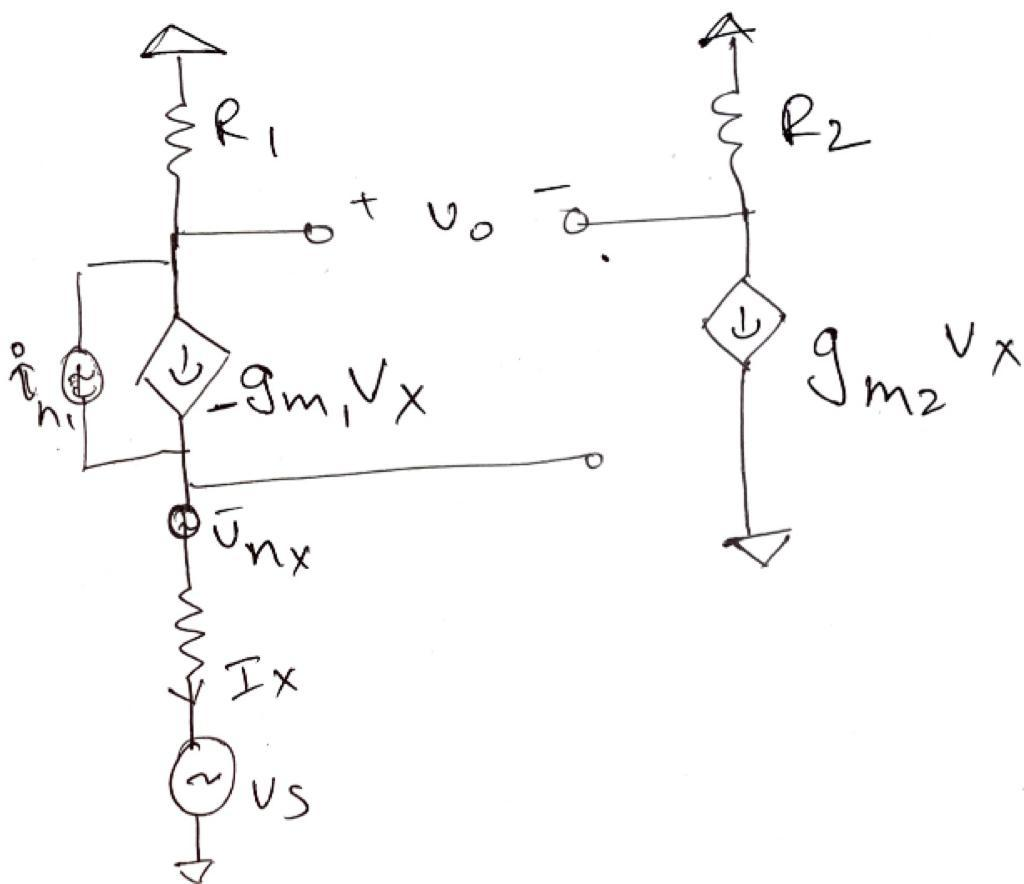
\includegraphics[scale=0.25]{./figs/q4.jpeg}
\end{figure}
\begin{gather*}
	V_x = V_s + R_sI_x = V_s - g_{m1}V_xR_s1\\
	\implies V_x = \frac{V_s}{1+g_{m1}R_s}\\
	I_x = -g_{m1}V_x
\end{gather*}
Input impedance here is $-V_x/I_x = 1/g_{m1}$. So if $\tcbhighmath[drop fuzzy shadow]{R_s = 1/g_{m1}}$ then the input is matched.
\begin{gather*}
	V_o = (g_{m1}R_1 + g_{m2}R_2)V_x\\
	\implies V_o = \frac{g_{m1}R_1 + g_{m2}R_2}{1+g_{m1}R_s}V_s\\
	\tcbhighmath[drop fuzzy shadow]{Gain = \frac{g_{m1}R_1 + g_{m2}R_2}{1+g_{m1}R_s}}
\end{gather*}
Now we find gains due to some noise causing elements,
\begin{gather*}
	\frac{\partial V_o}{\partial V_{n,x}} = g_{m1}R_1 + g_{m2}R_2\\
	\frac{\partial V_o}{\partial V_{n, R_1}} = 1\\
	\frac{\partial V_o}{\partial V_{n, R_2}} = -1\\
	\frac{\partial V_o}{\partial i_{n2}} = -R_2\\
\end{gather*}
To find the gain through M1, this changes $V_x$ and in turns $V_{o-}$ changes along with $V_{o+}$.
\begin{gather*}
	\Delta V_{o+} = i_{n1}R_1\\
	\Delta V_{o-} = g_{m2}i_{n1}R_sR_2\\
	\implies \frac{\partial V_o}{\partial i_{n1}} = R_1 - g_{m2}R_2R_s
\end{gather*}
To nullify the gain we need $\tcbhighmath[drop fuzzy shadow]{R_2 = \frac{R_1}{g_{m2}R_s} = \frac{1}{g_{m1}g_{m2}R_s}}$.
\begin{gather*}
	NF = \frac{4KTR_s + 4KTR_1 + 4KTR_2 + 4KTr_2g_{m2}R_2^2 + 4KTr_1g_{m1}(R_1 - g_{m2}-R_2R_s)^2}{4KTR_s}\\
	\implies \tcbhighmath[drop fuzzy shadow]{NF = 1 + \frac{R_1}{R_s} + \frac{\gamma g_{m2}R_2^2}{R_s} + \frac{\gamma g_{m1}(R_1 - g_{m2}R_2R_s)^2}{R_s}}
\end{gather*}
\section*{\hfil Problem 6}
\subsection*{(a)}
\begin{figure}[H]
	\centering
	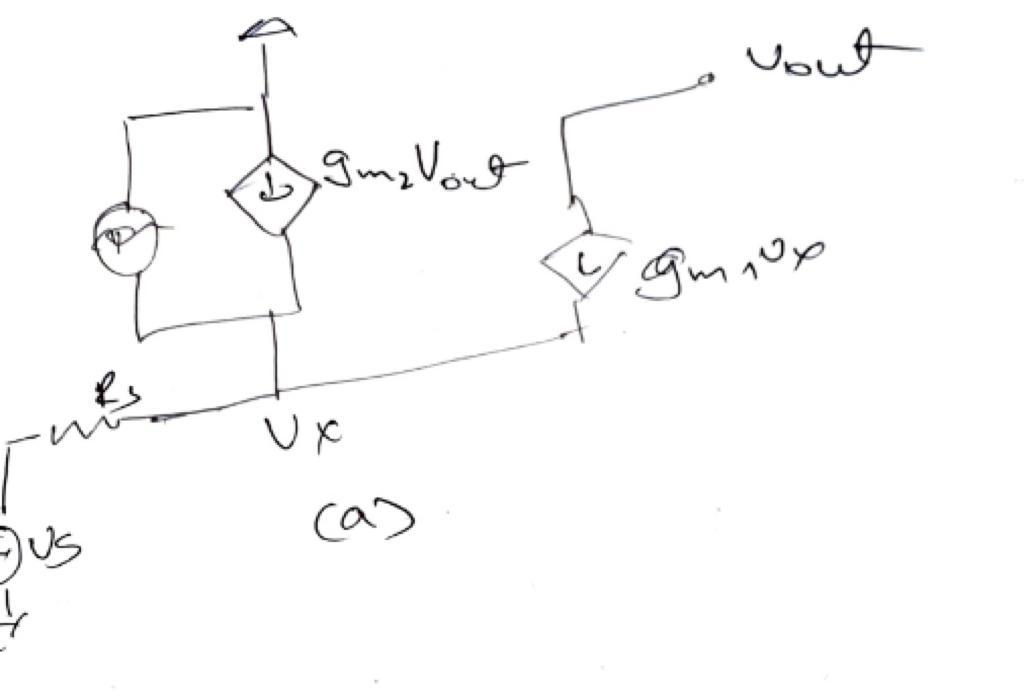
\includegraphics[scale=0.25]{./figs/q6a.jpeg}
\end{figure}
Clearly here noise generated by M2 must be compensated with small signal,\\
\begin{gather*}
	g_{m2}V_{o} = i_{n2} \implies V_{o}/i_{n2}=1/g_{m2}
\end{gather*}
Since there is no gain by M1,
\begin{gather*}
	NF = 1 + \gamma g_{m2}R_s
\end{gather*}
\subsection*{(b)}
\begin{figure}[H]
	\centering
	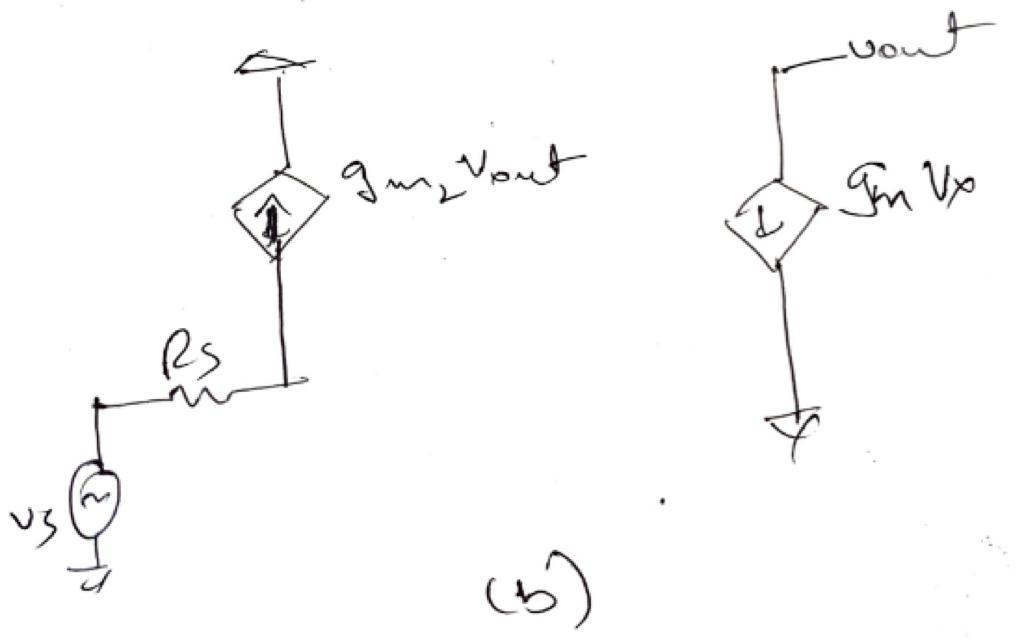
\includegraphics[scale=0.25]{./figs/q6b.jpeg}
\end{figure}
Here also it is the same case as before,
\begin{gather*}
	NF = 1 + \gamma g_{m2}R_s
\end{gather*}
\subsection*{(c)}
\begin{figure}[H]
	\centering
	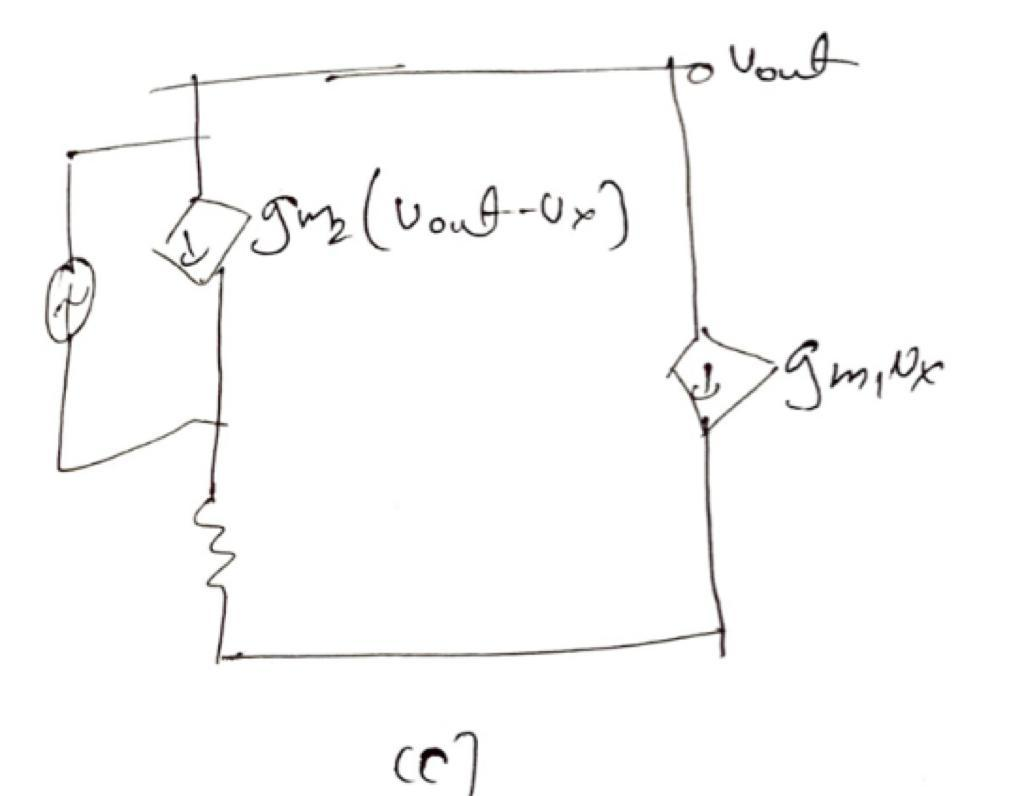
\includegraphics[scale=0.25]{./figs/q6c.jpeg}
\end{figure}
\subsection*{(d)}
\begin{figure}[H]
	\centering
	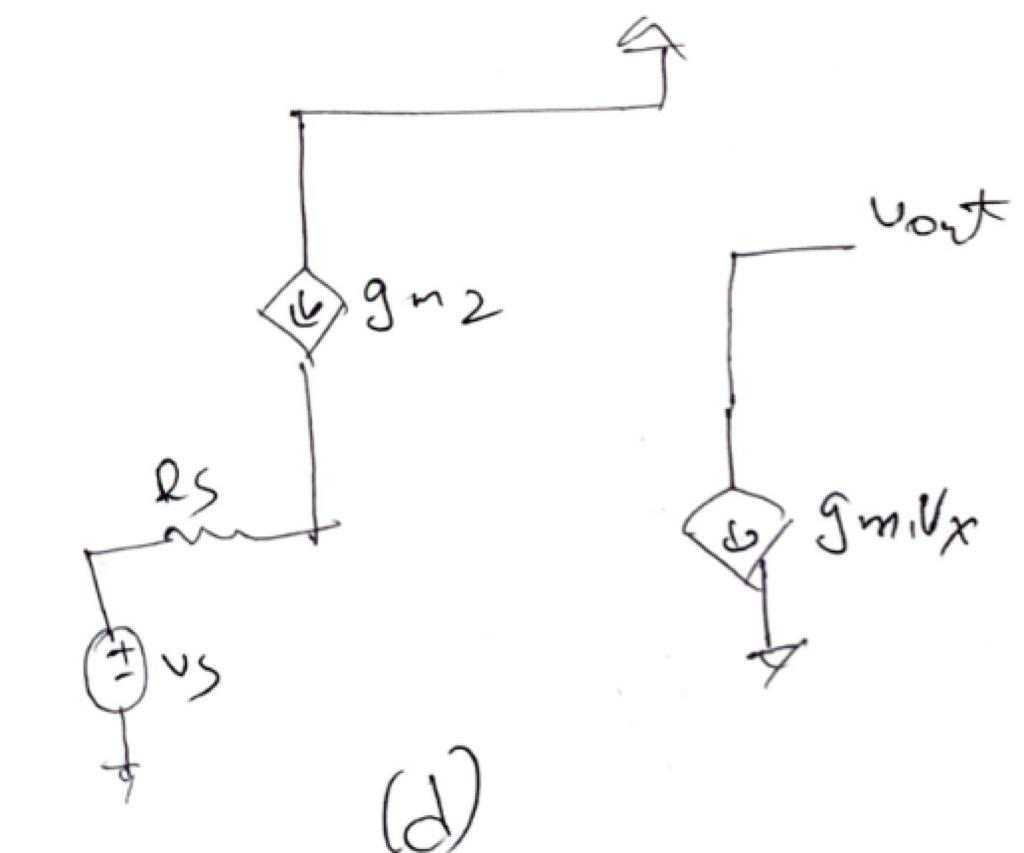
\includegraphics[scale=0.25]{./figs/q6d.jpeg}
\end{figure}
Here apart from M2 even M1 comes into picture because of drain and source connection,
\begin{gather*}
	NF = 1 + \gamma g_{m2}R_s + \frac{\gamma}{g_{m1}R_s}
\end{gather*}

\end{document}